\vvv\vvv\vvv
\presec
\subsection{Finding Super-spreaders} \postsec
\label{sec:basicAlgorithm:SS}

\ppp{Data Structure:}
In the data structure of InterestSketch for finding super-spreaders, both of the filter and the min-heap are used.  

For a given source IP address, we need to count the number of connections, \ie, the number of different destination IP addresses. 
%
If the source IP address sends more than one packet to a specific destination IP address, we increment the value of connection for only the first packet (but not for the other packets as these are duplicates in this case).
%
{
\color{reviewD}
%The Bloom filter is used for de-duplication before inserting items into the min-heap. 
We remind readers that details about Bloom filters are provided in Section~\ref{sub:findinterest}.
}


%
Each node in the min-heap stores two fields: the source IP address (ID) as key, and the \textit{connection} as value. 
%
The root node in the min-heap stores the source IP with the smallest connections.

{\color{reviewD}
\ppp{Insertion:}
The insertion process of finding Super-Spreaders is similar to that of our framework (Section \ref{sub:findinterest}).
%Given an incoming packet $e$, there are two steps. First we check the Bloom filter to judge whether $e$ is a duplicate. Second, if the Bloom filter reports true, $e$ is discarded. Otherwise, we try to insert $e$ into the min-heap.
There are two differences.
First, when checking or querying the Bloom filter, the item ID is the source IP address plus the destination IP address.
Second, when checking or updating the min-heap, the item ID is the source IP address only.
%Specifically, given an incoming packet $e$ (with ID of source+destination), we first check the Bloom filter by calculating the $z$ hash functions and get $z$ \textbf{\textit{hashed bits}}. 
%If all the $z$ hashed bits are 1, the packet is probably not the first one sent from the source to the specific destination, and it is discarded. 
%If the $z$ hashed bits are not all 1s, $e$ is definitely the first packet from the source to the destination. In this case, we first set all the $z$ bits to 1, and then try to insert $e$ (with ID of source only) into the min-heap. There are two cases: 1) If the source IP address of the packet is in the min-heap, we increment the corresponding connection. 2) Otherwise, if the min-heap is not full, we simply insert this source IP address into the min-heap. If the min-heap is full, we try to insert the source IP address into the root node by using our PRI algorithm.
}

{\color{reviewD}
\ppp{Report:}
The process of reporting Super-Spreaders is similar to that of Section \ref{sub:findinterest}.
%To report the source IP addresses above a given threshold $\mathcal{T}$, we traverse the min-heap to pick the source IP addresses with connection larger than $\mathcal{T}$.
}

\begin{comment}
\begin{figure}[htbp]
	\centering
	\prefig
	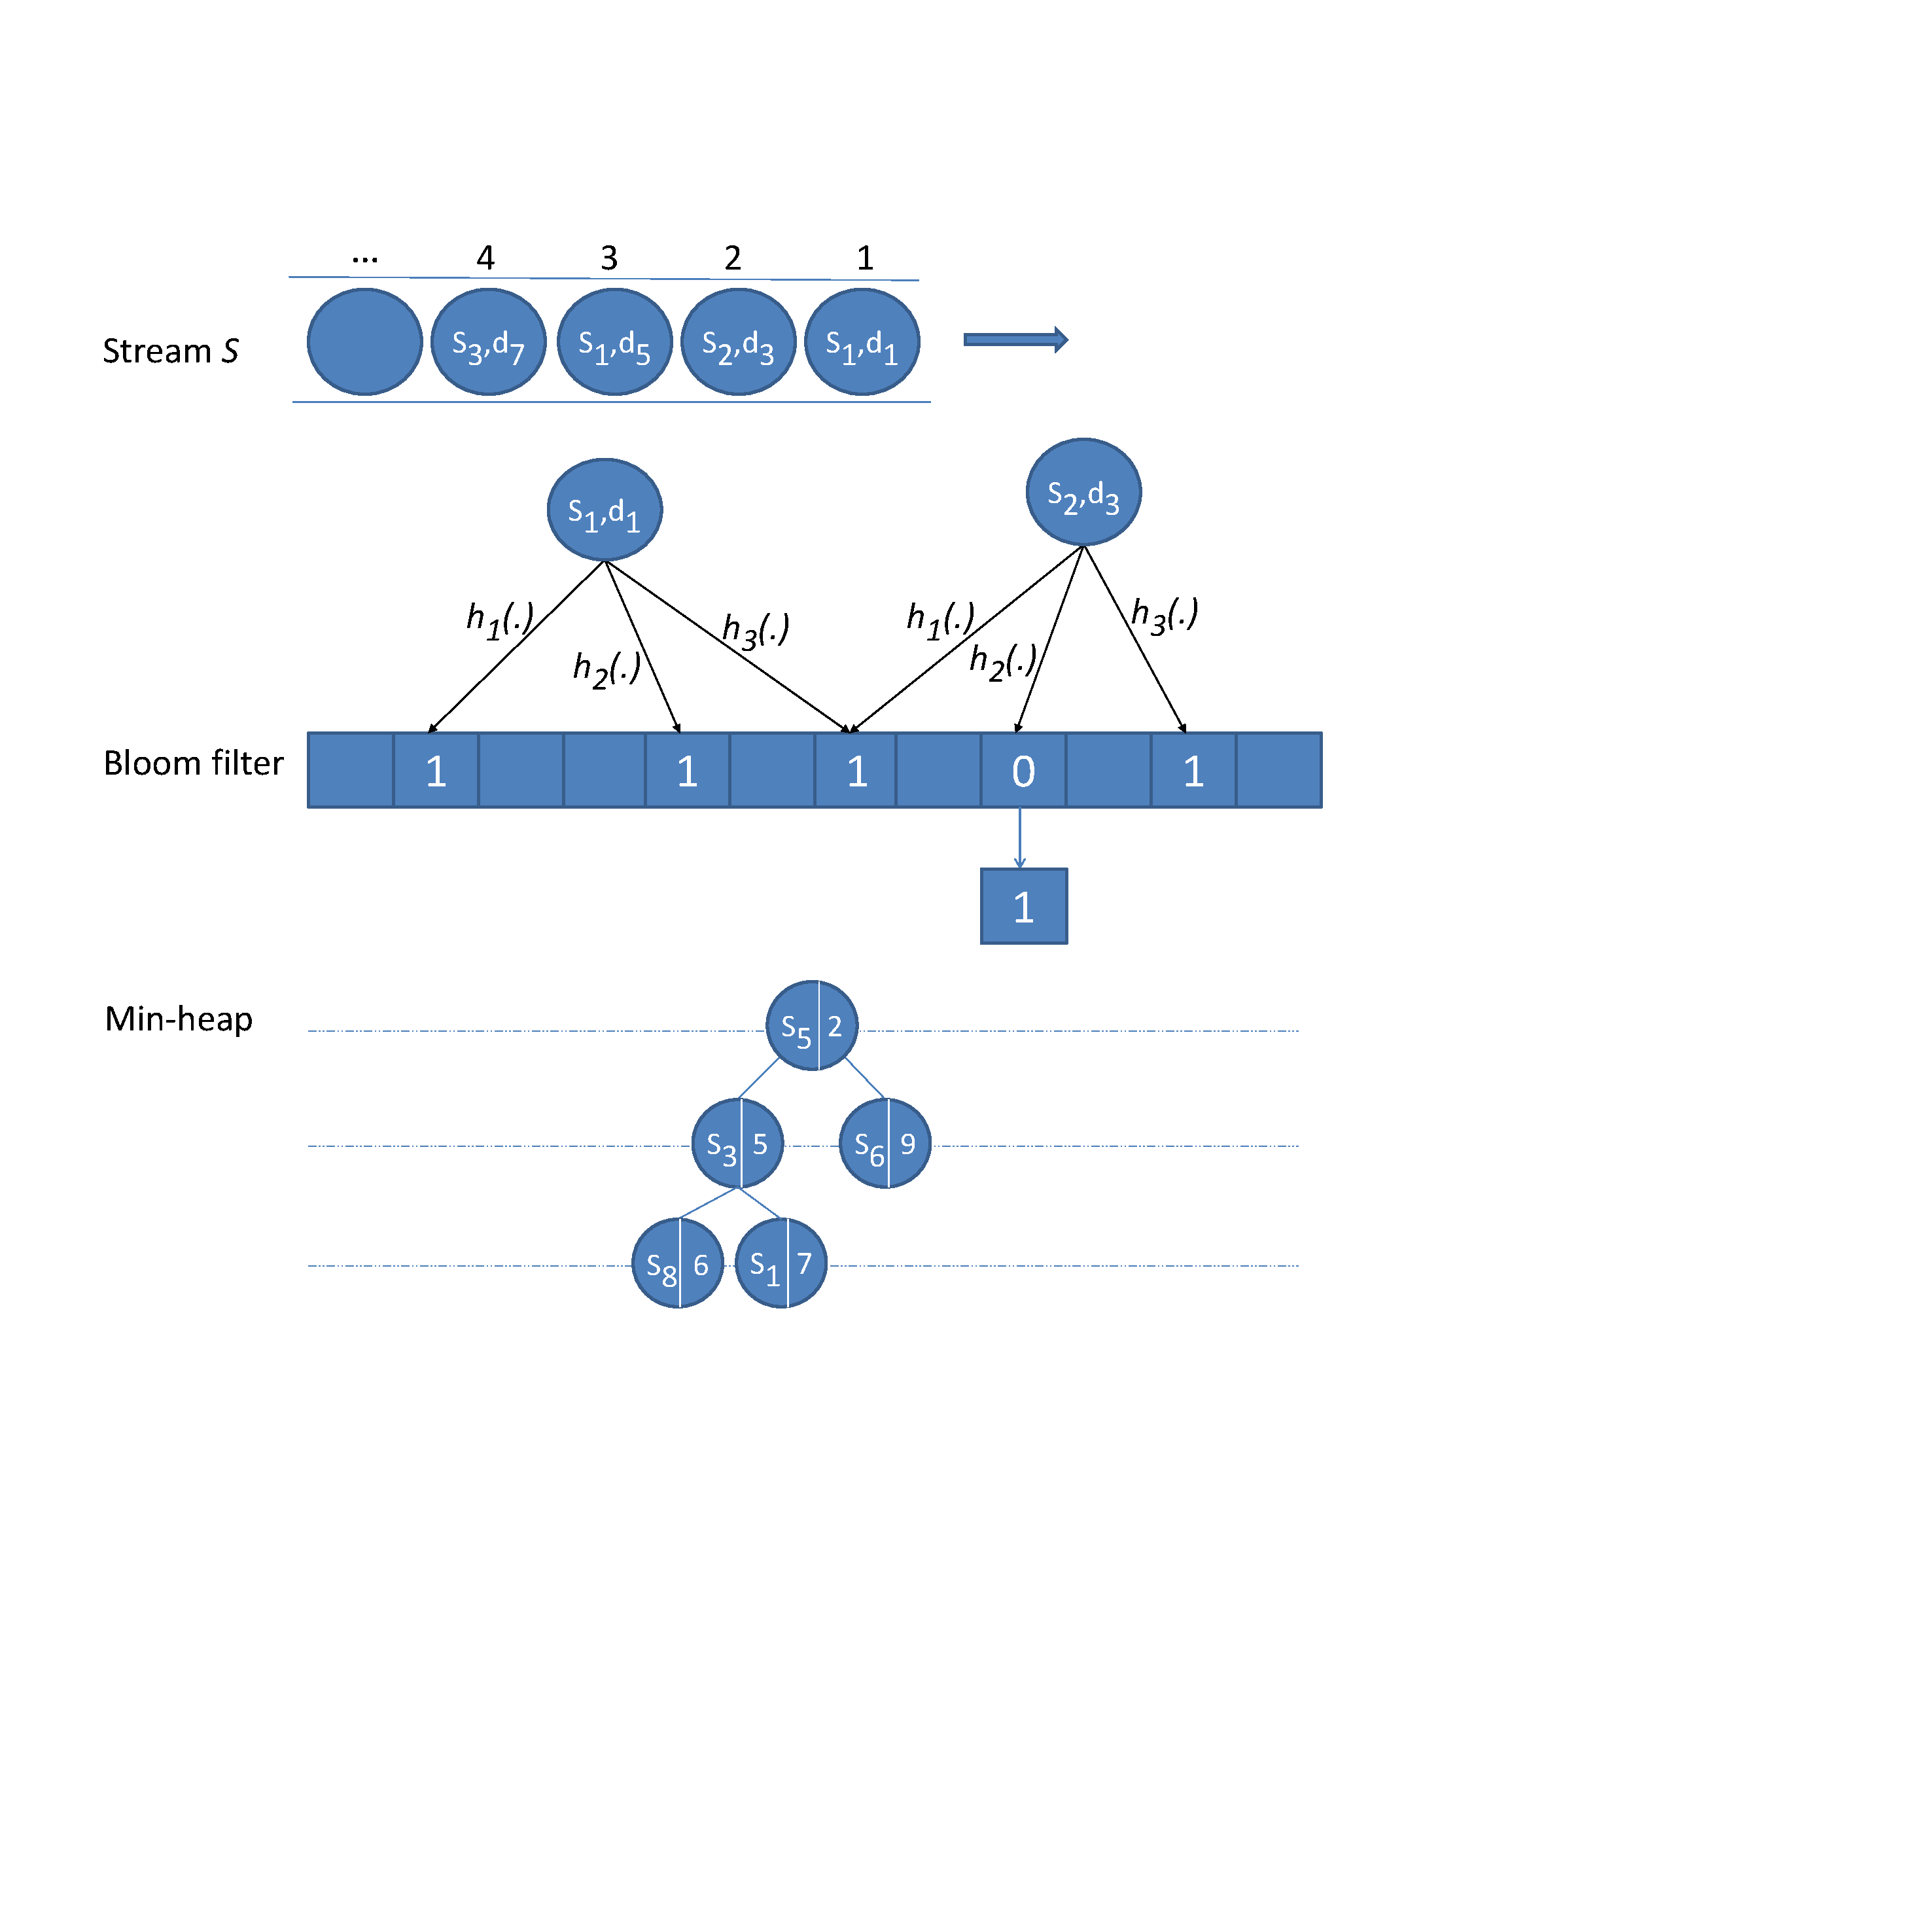
\includegraphics[width=0.5\textwidth]{GraphPPT/example_SS}
	\prefigcaption \vvv\vvv\vvv
	\caption{\aname{} for finding super-spreaders.}
	\label{draw:SS}
	\postfig \vvv\vvv \vvv\vvv
\end{figure}

\ppp{Example:}
As shown in Figure~\ref{draw:SS}, in the min-heap, the source IP address is stored in each node as the item ID. 
%
Given a network stream, each packet has a source IP address ($s_i$) and a destination IP address ($d_i$). 
%
For the first incoming packet with ($s_1,d_1$), we calculate three hash functions $h_1(s_1,d_1),h_2(s_1,d_1),~and~h_3(s_1,d_1)$. 
%
If all of three \textit{hashed bits} are $1$, indicating that this packet is not the first one sent from $s_1$ to $d_1$, we discard it. 
%
When the second packet with ($s_2$, $d_3$) arrives, one of the three hashed bits is $0$, indicating that this packet is the first one sent from $s_1$ to $d_3$ and $s_1$ is not in the min-heap. 
%
We change the second hashed bit from $0$ to $1$ in the Bloom filter and then insert $s_2$ into the min-heap, by applying our PRI algorithm (see Section \ref{sub:findfreq}). 
%
In this way, the source IP addresses with the largest connection (\ie, number of destination IP addresses) are recorded in the min-heap. 
%
%The algorithm is shown in Algorithm~\ref{alg:sup} in Appendix~\ref{sec:appendix}.
%
The detailed description of the algorithm is similar to the basic Algorithm.
%~\ref{alg:basic}.

\end{comment}